\section{Langzeitwirkung: Die Erzählung der De-Industrialisierung und das Leben im Anthropozän}

\subsection{Einführung: De-Industrialisierung und Langzeitwirkungen}

Die Vorlesung untersucht die Erzählung
der De-Industrialisierung
und verbindet sie mit der Frage,
wie technische Systeme langfristig
soziale,
räumliche
und ökologische Wirkungen entfalten.

Im Zentrum steht nicht nur die Frage,
ob Industrie verschwindet.

Entscheidend ist vielmehr,
was von industriellen Gesellschaften bleibt,
wenn Fabriken,
Zechen
oder industrielle Arbeitsplätze geschlossen werden.

De-Industrialisierung bedeutet daher nicht einfach
das Ende der Industrie.

Sie beschreibt vielmehr eine Verschiebung
industrieller Produktion,
die Auflösung bestimmter sozialer Ordnungen
und das Nachleben technischer Systeme.

Zentrale Leitfragen:

\begin{itemize}
\item Was bedeutet De-Industrialisierung?
\item Warum erscheint seit den 1970er Jahren das Ende der Industriegesellschaft plausibel?
\item Welche Rolle spielen Angestellte, Automatisierung, Globalisierung und Neoliberalismus?
\item Was bleibt von Industrie nach ihrer Stilllegung?
\item Wie wirken technische Systeme im Anthropozän langfristig weiter?
\end{itemize}

Die Vorlesung zeigt,
dass industrielle Technik nicht einfach endet,
wenn industrielle Arbeit verschwindet.

Ihre Spuren bleiben in Landschaften,
Infrastrukturen,
sozialen Milieus,
politischen Konflikten
und ökologischen Belastungen erhalten.

\subsection{Ölschiefer-Abbau im Nordosten Estlands}

Ein zentrales Beispiel der Vorlesung
ist der Ölschiefer-Abbau im Nordosten Estlands.

Die Region um Kiviõli
war seit den 1920er Jahren
eine wichtige Industrieregion,
besonders während der Sowjetzeit.

Ölschiefer ist ein Gestein,
das organisches Material namens Kerogen enthält.

Dieses entstand vor Millionen von Jahren
aus abgestorbenen Algen und Mikroorganismen.

Durch Verschwelung kann aus Ölschiefer
Öl gewonnen werden.

Dazu wird das Gestein abgebaut,
zerkleinert
und unter Sauerstoffausschluss stark erhitzt.

Typischerweise geschieht dies bei Temperaturen
von etwa 450 bis 500 Grad Celsius.

Dabei zerfällt das Kerogen chemisch.

Es entstehen:

\begin{itemize}
\item flüssige Kohlenwasserstoffe
\item Schieferöl
\item brennbare Gase
\item Rückstände aus Kohlenstoff und Mineralien
\end{itemize}

Die Dämpfe werden anschliessend abgekühlt,
sodass ein rohes Öl entsteht,
das ähnlich wie Erdöl weiter raffiniert werden kann.

\subsection{Industrialisierung, Sowjetzeit und sozialer Umbruch}

Der Ölschiefer-Abbau machte den Nordosten Estlands
zu einer zentralen Industrieregion.

Während der Sowjetzeit
wurden viele russischsprachige Arbeiterinnen und Arbeiter
in der Region angesiedelt.

Die industrielle Struktur
prägte daher nicht nur die Wirtschaft,
sondern auch Bevölkerung,
Sprache,
Arbeitswelt
und regionale Identität.

Nach dem Zusammenbruch der Sowjetunion um 1990
kam es zu einem tiefgreifenden Strukturwandel.

Die sowjetischen Absatz-
und Versorgungsstrukturen brachen zusammen.

Es folgten Rationalisierung,
Schliessungen
und Arbeitsplatzverluste.

Die Region erlebte einen raschen sozialen
und demographischen Rückgang.

De-Industrialisierung bedeutete hier also nicht nur,
dass bestimmte Produktionsformen verschwanden.

Sie bedeutete auch den Verlust
einer sozialen Ordnung,
die auf industrieller Arbeit,
staatlicher Planung
und regionaler Zugehörigkeit beruhte.

\begin{center}
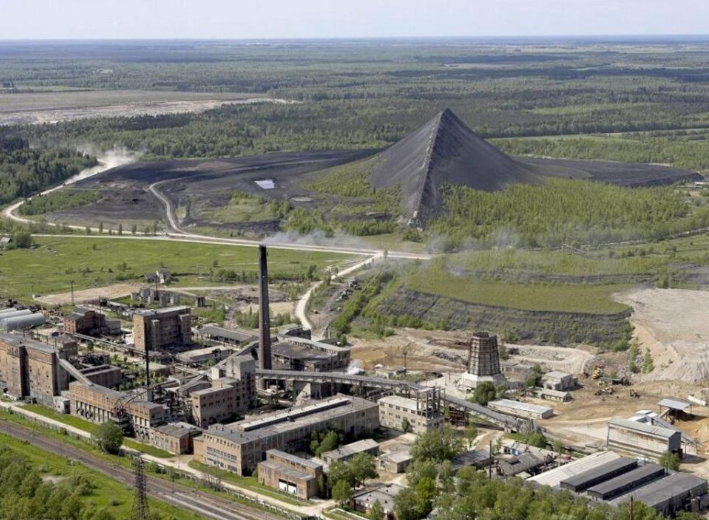
\includegraphics[width=0.8\linewidth]{images/oelschiefer_estland.png}
\end{center}

\subsection{Industrie als Nachleben}

Die Landschaft im Nordosten Estlands
bleibt bis heute industriell geprägt.

Auch wenn industrielle Produktion zurückgeht
oder sich verändert,
verschwinden ihre Spuren nicht.

Zurück bleiben:

\begin{itemize}
\item Gruben
\item Kraftwerke
\item industrielle Infrastrukturen
\item Abraumhalden
\item belastete Böden
\item transformierte Landschaften
\end{itemize}

Das Kiviõli Adventure Center
steht exemplarisch für dieses industrielle Nachleben.

Es befindet sich auf einem Berg
aus Abfällen der Ölschieferindustrie.

Dieser Berg glüht in seinem Innern
weiterhin auf rund 80 Grad Celsius.

Die frühere Industrielandschaft
wird nun touristisch genutzt,
etwa durch Freizeitparks,
Abenteuerferien
und Veranstaltungsorte.

Solche Nutzungen können als Industriearchäologie
oder als Versuch verstanden werden,
wirtschaftliche Alternativen aufzubauen.

Gleichzeitig bleiben soziale
und wirtschaftliche Fragilität bestehen.

Die Industrie ist daher nicht einfach abgeschlossen.

Sie lebt als Landschaft,
Infrastruktur,
Risiko
und Erinnerung weiter.

\begin{center}
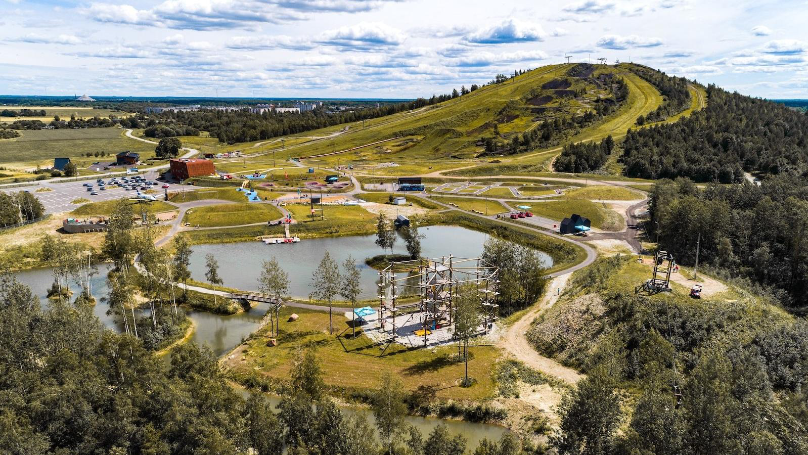
\includegraphics[width=0.8\linewidth]{images/kivioli_adventure_center.png}
\end{center}

\subsection{Das Ende der Industriegesellschaft?}

Seit den 1970er Jahren
entstand in westlichen Gesellschaften
zunehmend der Eindruck,
das industrielle Zeitalter gehe zu Ende.

Mehrere Entwicklungen schienen
auf einen Übergang
in eine neue Gesellschaftsform hinzuweisen.

Dazu gehörten:

\begin{itemize}
\item Rückgang klassischer Industriearbeit
\item Bedeutungsverlust der klassischen Arbeiterklasse
\item Schliessung von Zechen und Fabriken
\item Wachstum des Dienstleistungssektors
\item Wachstum von Verwaltung, Finanzwirtschaft und Bildung
\item Aufstieg von Informationstechnologie
\item Zunahme von Angestellten- und Wissensarbeit
\end{itemize}

Die westlichen Gesellschaften schienen
in ein postindustrielles,
wissensbasiertes
oder informationsbasiertes Zeitalter einzutreten.

Begriffe wie Wissensgesellschaft,
Informationsgesellschaft
oder Netzwerkgesellschaft
wurden Ausdruck dieser Erwartung.

Technische Entwicklungen wie Automatisierung,
politische Entwicklungen wie Neoliberalismus
und sozioökonomische Entwicklungen wie Globalisierung
verstärkten diesen Eindruck.

\subsection{De-Industrialisierung als Erzählung}

De-Industrialisierung bezeichnet
nicht nur konkrete historische Entwicklungen.

Sie ist auch eine gesellschaftliche Erzählung.

Diese Erzählung wurde durch öffentliche Diskussionen
in unterschiedliche Richtungen gedeutet.

Einerseits gab es eine euphorische Deutung.

Das Ende der Schwerindustrie
wurde als Übergang
in ein neues,
modernes
und scheinbar sauberes Zeitalter verstanden.

Industrie erschien dabei als alt,
schmutzig
und überholt.

Informationstechnologie,
Dienstleistungsarbeit
und Wissensarbeit galten dagegen
als Zukunft.

Andererseits gab es eine pessimistische Deutung.

Hier erschien De-Industrialisierung
als soziale Krise.

Im Zentrum standen:

\begin{itemize}
\item Verlust von Arbeit
\item Verlust von Identität
\item Bedeutungsverlust ganzer Regionen
\item Arbeitslosigkeit
\item politische Entfremdung
\item soziale Verarmung
\end{itemize}

Die Erzählung der De-Industrialisierung
war daher ambivalent.

Sie konnte Fortschritt versprechen,
aber auch Niedergang,
Verlust
und Krise bedeuten.

\subsection{Die Angestellten als Produkt der Industrialisierung}

Ein wichtiger Teil dieser Geschichte
ist die Entstehung des modernen Angestelltentums.

Angestellte entstanden nicht erst
nach der Industriegesellschaft.

Sie sind selbst ein Produkt
der Industrialisierung des 19. Jahrhunderts.

Mit wachsender industrieller Produktion
entstanden neue Anforderungen
an Verwaltung,
Planung,
Buchhaltung,
Kommunikation
und technische Koordination.

Grosse Unternehmen,
Eisenbahnen,
Banken,
Versicherungen
und Staatsverwaltungen
benötigten zunehmend Personal,
das nicht direkt an der Maschine arbeitete.

Diese Personen organisierten,
verwalteten
und koordinierten industrielle Prozesse.

Das Angestelltentum war daher
eng mit der Industriegesellschaft verbunden,
auch wenn es sich häufig
von der Arbeiterschaft abgrenzte.

\subsection{Technisierung des Büros}

Das moderne Angestelltentum entstand
zusammen mit neuen Technologien
der Informationsverarbeitung.

Dazu gehörten:

\begin{itemize}
\item Schreibmaschinen
\item Telefone
\item Karteisysteme
\item Rechenmaschinen
\item standardisierte Formulare
\item später Computer und Datenverarbeitung
\end{itemize}

Die industrielle Produktion
musste nicht nur hergestellt,
sondern auch geplant,
verwaltet
und koordiniert werden.

Dafür brauchte es bürokratische Bereiche.

Diese umfassten etwa:

\begin{itemize}
\item Korrespondenz mit Kunden
\item Kontakt zu Abnehmern und Verkäufern
\item Handel und Vertrieb
\item Statistik
\item Marktbeobachtung
\item Produktionsplanung
\end{itemize}

Die Anpassungsfähigkeit der Produktion
wurde zunehmend marktrelevant.

Dafür brauchte es Überblick,
eingespielte Verfahren
und Informationsverarbeitung.

Das Büro war daher kein Gegensatz
zur Industrie.

Es war eine Voraussetzung
für deren komplexe Organisation.

\subsection{Identität und Zugehörigkeit der Angestellten}

Angestellte waren zwar lohnabhängig,
verstanden sich historisch jedoch häufig
nicht als Teil der Arbeiterschaft.

Sie entwickelten eigene Selbstbilder
und soziale Abgrenzungen.

Typische Selbstbilder waren:

\begin{itemize}
\item geistige statt körperliche Arbeit
\item Bildung und Respektabilität
\item Individualität
\item Aufstiegsorientierung
\item Nähe zu Verwaltung, Technik und Management
\end{itemize}

Sozial grenzten sich Angestellte
häufig nach unten
von der Arbeiterschaft ab.

Gleichzeitig orientierten sie sich nach oben
an bürgerlichen Lebensformen.

Dadurch verkomplizierte das Angestelltentum
den klassischen Gegensatz
zwischen Bourgeoisie und Proletariat.

Gesellschaftliche Konflikte
liessen sich nicht mehr nur
als Klassenkampf zwischen Arbeiterschaft
und Besitzbürgertum beschreiben.

\begin{center}

\includegraphics[width=0.75\linewidth]{images/angestellte_identitaet.png}
\end{center}

\subsection{Angestellte und De-Industrialisierung}

Die Orientierung des Angestelltentums
hatte Auswirkungen auf das politische
und gesellschaftliche Gefüge.

Sie trug dazu bei,
bürgerliche Lebensstile
über die eigentliche bürgerliche Bevölkerungsschicht hinaus
zu verbreiten.

In den 1970er Jahren
lösten Angestellte die Arbeiterschaft
jedoch nicht einfach als soziale Gruppe ab.

Vielmehr verschob sich die symbolische Bedeutung.

Während der Industriearbeiter lange
als zentrale Figur moderner Produktion galt,
erschienen seit den 1970er Jahren
zunehmend Angestellte,
Verwaltungsarbeiter
und Wissensarbeiter
als repräsentativ für die Zukunft
westlicher Gesellschaften.

Der Angestellte erschien nun
als geeigneter Träger
einer neuen Wirtschaftsordnung.

Diese schien weniger auf sichtbare,
körperliche Produktion ausgerichtet zu sein
als auf Organisation,
Kommunikation
und Informationsverarbeitung.

\subsection{Automatisierung und Computerisierung}

Computerisierung und Automatisierung
veränderten industrielle Produktionsprozesse
grundlegend.

Tätigkeiten wurden standardisiert,
technisch reorganisiert
und datenbasiert koordiniert.

Industriearbeit verschwand dadurch jedoch nicht einfach.

Computer ersetzten den Industriearbeiter
oder die Industriearbeiterin nicht vollständig.

Sie veränderten vielmehr,
welche Fähigkeiten
und Qualifikationen
erforderlich wurden.

Bestimmte Formen industrieller Arbeit
verloren an Bedeutung,
während neue technische,
organisatorische
und kontrollierende Tätigkeiten wichtiger wurden.

Automatisierung bedeutete daher
nicht das Ende von Arbeit,
sondern ihre Neuordnung.

\subsection{Globalisierung und räumliche Entkopplung}

Neben der Automatisierung spielte
die Globalisierung eine zentrale Rolle.

Produktion wurde zunehmend global organisiert.

Unternehmen verlagerten:

\begin{itemize}
\item Fertigung
\item Rohstoffgewinnung
\item Montage
\item Zulieferketten
\item arbeitsintensive Produktionsschritte
\end{itemize}

Dadurch entstand eine politische Konkurrenz
zwischen Staaten.

Diese konkurrierten etwa um:

\begin{itemize}
\item niedrige Steuern
\item günstige Arbeitsbedingungen
\item schwächere Regulierungen
\item geringere Umweltauflagen
\end{itemize}

Die Folge war die De-Industrialisierung
vieler westlicher Industrieregionen.

Klassische Industriearbeitsplätze gingen verloren.

Zugleich wurden Konsum,
Verwaltung
und Produktion räumlich voneinander getrennt.

Industrie verschwand dadurch nicht an sich.

Sie verschwand vor allem
aus dem unmittelbaren Blickfeld
westlicher Gesellschaften.

\subsection{Die neoliberale Wende}

Ein weiterer wichtiger Faktor
war die neoliberale Wende.

Nach 1945 entstand in vielen westlichen Staaten
eine Form sozialstaatlich regulierten Kapitalismus.

Diese beruhte auf:

\begin{itemize}
\item Massenproduktion
\item Massenkonsum
\item Tarifpartnerschaft
\item relativ stabiler Industriearbeit
\item sozialstaatlicher Absicherung
\end{itemize}

Die Industriegesellschaft wurde politisch stabilisiert.

Dies geschah nicht nur aus ökonomischen Gründen.

Es ging auch darum,
sozialen Frieden zu sichern.

Wichtige Hintergründe waren:

\begin{itemize}
\item die Erinnerung an Faschismus und Weltwirtschaftskrise
\item die Stärke der Gewerkschaften
\item die Vermeidung von Klassenkampf
\item der Kalte Krieg und die Konkurrenz zum Staatssozialismus
\end{itemize}

Industriepolitik war damit auch Gesellschaftspolitik.

Sie versprach Vollbeschäftigung,
regionale Stabilität
und politische Befriedung.

\subsection{Auflösung des Nachkriegsarrangements}

Das Nachkriegsarrangement
zwischen Arbeitgeberinnen,
Arbeitgebern,
Arbeitnehmerinnen
und Arbeitnehmern
bedeutete eine künstliche Stabilisierung
industrieller Gesellschaften.

In den 1970er Jahren
wurde dieses Arrangement zunehmend in Frage gestellt.

Gründe dafür waren unter anderem:

\begin{itemize}
\item Ölkrisen
\item zunehmende internationale Konkurrenz
\item Automatisierung
\item Globalisierung
\item Arbeitslosigkeit
\item Finanzialisierung
\end{itemize}

Globalisierung reduzierte lokale Abhängigkeiten.

Technische Umstrukturierung
veränderte Produktionsweisen.

Arbeitslosigkeit schwächte Gewerkschaften.

Finanzialisierung veränderte Unternehmenslogiken.

Die wirtschaftlichen und politischen Bedingungen
veränderten sich so,
dass der soziale Kompromiss der Nachkriegszeit
zunehmend aufgekündigt wurde.

Besonders deutlich wurde dies
in Thatchers Grossbritannien
und Reagans USA.

\subsection{Britische Bergarbeiterstreiks 1984/85}

Ein zentrales Beispiel für die neoliberale Wende
sind die britischen Bergarbeiterstreiks
von 1984 und 1985.

Die Regierung Thatcher wollte
unrentable Zechen schliessen
und Subventionen abbauen.

Damit verband sie auch das Ziel,
die Macht der Gewerkschaften
in der britischen Politik zu brechen.

Die Wirtschaft sollte grundlegend umgebaut werden.

Dieser Umbau richtete sich gegen
das sozialstaatlich stabilisierte
Nachkriegsarrangement.

Als Thatcher 1984
die Schliessung zahlreicher Zechen beschloss,
traten mehr als 150 000 Bergarbeiter
für fast ein Jahr in den Streik.

Organisiert wurde der Streik
von der National Union of Mineworkers.

Es handelte sich um den grössten Arbeiterstreik
der britischen Nachkriegszeit.

\begin{center}

\includegraphics[width=0.75\linewidth]{images/thatcher_bergarbeiterstreik.png}
\end{center}

\subsection{Der Bergarbeiterstreik als Kampf um Lebensformen}

Der Kohlebergbau hatte in Regionen
wie Yorkshire,
Wales,
den Midlands,
Nordengland
und Schottland
eine Bedeutung,
die weit über die reine Wirtschaft hinausging.

Er prägte:

\begin{itemize}
\item lokale Gemeinschaften
\item Geschäfte
\item politische Identitäten
\item Wohnungsbau
\item Gewerkschaftskulturen
\item regionale Zugehörigkeit
\end{itemize}

Die Bergarbeiter verstanden den Konflikt
daher nicht nur als Arbeitskampf.

Sie sahen ihn als Kampf
um Lebensformen,
um das Überleben ganzer Industriestandorte,
um regionale Gemeinschaften
und um politische Würde.

Der Streik endete jedoch
mit einer Niederlage der Bergarbeiter.

Viele Zechen wurden geschlossen.

Die Macht der Gewerkschaften
brach massiv ein.

Auch die Überzeugung,
dass die lokale Arbeiterschaft nötig sei,
um die Wirtschaft am Laufen zu halten,
wurde geschwächt.

\subsection{Langzeitfolgen der De-Industrialisierung}

Langfristig beschleunigte die Niederlage
der britischen Bergarbeiter
die De-Industrialisierung
vieler Industrieregionen.

Die Folgen waren tiefgreifend.

Dazu gehörten:

\begin{itemize}
\item Massenarbeitslosigkeit
\item soziale Verarmung
\item politische Entfremdung
\item langfristige regionale Ungleichheit
\item schlechte Infrastruktur
\item Gesundheitsprobleme
\item politische Radikalisierung
\item Perspektivlosigkeit
\end{itemize}

Diese Folgen verschwanden nicht
nach wenigen Jahren.

Viele ehemalige Bergbauregionen
kämpfen bis heute
mit den strukturellen Nachwirkungen
der De-Industrialisierung.

Damit wird deutlich,
dass De-Industrialisierung
nicht nur ein ökonomischer Prozess ist.

Sie verändert soziale Welten
und wirkt über Generationen weiter.

\begin{center}

\includegraphics[width=0.75\linewidth]{images/bergarbeiterstreik_1984_85.png}
\end{center}

\subsection{Mehr als De-Industrialisierung}

Was seit den 1970er Jahren geschah,
war in gewissem Sinne mehr
als De-Industrialisierung.

Denn es verschwanden nicht nur Arbeitsplätze.

Es verschwanden ganze soziale Welten.

Dazu gehörten:

\begin{itemize}
\item industrielle Identitäten
\item kollektive Lebensformen
\item regionale Zugehörigkeiten
\item politische Milieus
\item Gewerkschaften und Arbeiterbewegung
\item Zukunftserwartungen
\item kulturelle Selbstverständnisse
\end{itemize}

Nicht nur Arbeit verschwand,
sondern die industrielle Gesellschaft
als Erfahrungsraum.

Industrie war also nicht nur
eine Produktionsform.

Sie war auch eine soziale,
politische
und kulturelle Ordnung.

\subsection{Weniger als De-Industrialisierung}

Gleichzeitig war der Prozess
auch weniger als De-Industrialisierung.

Denn Industrie verschwand nicht einfach.

Industriepolitik gibt es weiterhin.

Auch heute existieren etwa
Autoindustrie,
Stahlindustrie,
Gewerkschaften,
Tarifverträge
und Verhandlungen zwischen Sozialpartnern.

Was sich veränderte,
war vor allem die räumliche,
soziale
und politische Konzentration der Industrie.

Produktion wurde verlagert,
Prozesse wurden automatisiert
und Wertschöpfungsketten wurden fragmentiert.

Industrie verschwand also nicht,
sondern wurde räumlich entkoppelt
und verlor an Sichtbarkeit.

De-Industrialisierung bezeichnet daher
weniger das Ende der Industrie
als die Auflösung ihrer lokalen,
sozialen
und politischen Konzentration.

\subsection{Leben im Anthropozän}

Die Vorlesung verbindet De-Industrialisierung
mit der Frage nach dem Leben im Anthropozän.

Das Anthropozän bezeichnet eine Gegenwart,
in der menschliche Eingriffe
geologische,
ökologische
und planetare Wirkung entfalten.

Technische Systeme prägen dabei
nicht nur unmittelbare Arbeitsprozesse.

Sie wirken langfristig weiter.

Wichtige Aspekte sind:

\begin{itemize}
\item normative Wirkung technischer Systeme
\item Irreversibilität technischer Eingriffe
\item Trägheit materieller Infrastrukturen
\item langfristige ökologische Folgen
\item Transformation von Landschaften
\item Veränderung von Stoffkreisläufen
\item soziale und kulturelle Nachwirkungen
\end{itemize}

Technik strukturiert Arbeit,
Verhalten
und Wahrnehmung
über ihre reine Funktion hinaus.

Sie prägt Alltagsroutinen,
Organisationen
und Erwartungen.

\subsection{Langzeitwirkung technischer Systeme}

Technische Systeme enden nicht
mit den Gesellschaften,
die sie hervorgebracht haben.

Ihre Wirkungen können ihre ursprünglichen
sozialen,
politischen
und ökonomischen Kontexte überdauern.

Industrieanlagen,
Infrastrukturen,
Bergwerke,
Abraumhalden
und belastete Landschaften
wirken weiter,
auch wenn die ursprüngliche Produktion
eingestellt wurde.

Solche Systeme sind träge.

Sie lassen sich nicht einfach abschalten
oder rückgängig machen.

Ihre Folgen können Generationen überdauern.

Das gilt sozial,
räumlich
und ökologisch.

Wenn man über De-Industrialisierung nachdenkt,
wird daher klar:

Industrie verschwindet nicht einfach.

Sie bleibt als Nachleben,
als Infrastruktur,
als ökologische Belastung,
als soziale Erinnerung
und als politische Folge bestehen.

\subsection{Zentrale Erkenntnisse}

Die Vorlesung zeigt,
dass De-Industrialisierung
nicht einfach das Ende der Industrie bedeutet.

Sie beschreibt vielmehr die Verschiebung
und Entkopplung industrieller Produktion
sowie den Verlust bestimmter sozialer,
politischer
und regionaler Ordnungen.

Zentrale Erkenntnisse sind:

\begin{itemize}
\item Industrie wirkt auch nach ihrer Stilllegung weiter.
\item De-Industrialisierung bedeutet nicht das vollständige Verschwinden von Industrie.
\item Industrie verliert vor allem ihre lokale, soziale und politische Konzentration.
\item Angestellte und Wissensarbeit entstehen selbst aus der Industrialisierung.
\item Automatisierung verändert Arbeit, ersetzt sie aber nicht einfach vollständig.
\item Globalisierung verschiebt Produktion aus dem Blickfeld westlicher Gesellschaften.
\item Die neoliberale Wende löste das Nachkriegsarrangement industrieller Stabilisierung auf.
\item De-Industrialisierung betrifft nicht nur Arbeitsplätze, sondern ganze Lebensformen.
\item Technische Systeme entfalten langfristige soziale, räumliche und ökologische Wirkungen.
\end{itemize}

Die zentrale These lautet:

De-Industrialisierung ist weniger das Ende der Industrie
als die Auflösung ihrer sichtbaren,
lokalen
und gesellschaftlich stabilisierten Form.

Industrie verschwindet nicht einfach.

Sie wird verlagert,
automatisiert,
fragmentiert
und bleibt zugleich als Nachleben bestehen.

Im Anthropozän zeigt sich,
dass technische Systeme
nicht mit ihren historischen Gesellschaften enden,
sondern als langfristige Strukturen weiterwirken.
